% ============================================================
% 4  Large N: why x^{2/3}, and the electron Green's function
% ============================================================
\begin{frame}[t]
\ft{Large $N$: why $x^{2/3}$}
\begin{columns}[T]
\begin{column}{0.52\textwidth}
\vspace{0.3cm}
{\small $N$ flavours,\ $\tfrac{\lambda_4}{4N}(\partial_x\phi\cdot\partial_x\phi)^2$\ $\Rightarrow$ saddle point\par}
\vspace{0.3cm}
{\small\colorbox{cLL!20}{\mystrut $e^{i\beta\theta}$}\ \ cost of the source saturates $\Rightarrow$ LRO\par}
\vspace{0.3cm}
\onslide<2->{%
{\small\colorbox{cQCP!15}{\mystrut $e^{i\beta\phi}$}\ \ source reshapes the saddle, $r\propto(\partial_xu)^4$\par}
\vspace{0.1cm}
\centering
{\small$\displaystyle \ln\chi_\phi\simeq-N\!\int\!\Big[fu-\tfrac12\colorbox{orchid!25}{$\mystrut(\partial_\tau u)^2$}-\tfrac{2\pi^2}{3}\colorbox{orchid!25}{$\mystrut(\partial_xu)^6$}\Big]$\par}}
\vspace{0.3cm}
\onslide<3->{%
\raggedright
{\small\colorbox{pumpkin!50}{\mystrut Power counting}\ \ $\tau\sim x^{5/3}$,\ $u\sim x^{2/3}$\par}
\vspace{0.1cm}
\centering
{\small$\displaystyle\Rightarrow\ \ln\chi_\phi\sim-N C\,|\beta|^{4/3}\,|x|^{2/3}$\par}}
\end{column}
\begin{column}{0.46\textwidth}
\centering
\vspace{0.4cm}
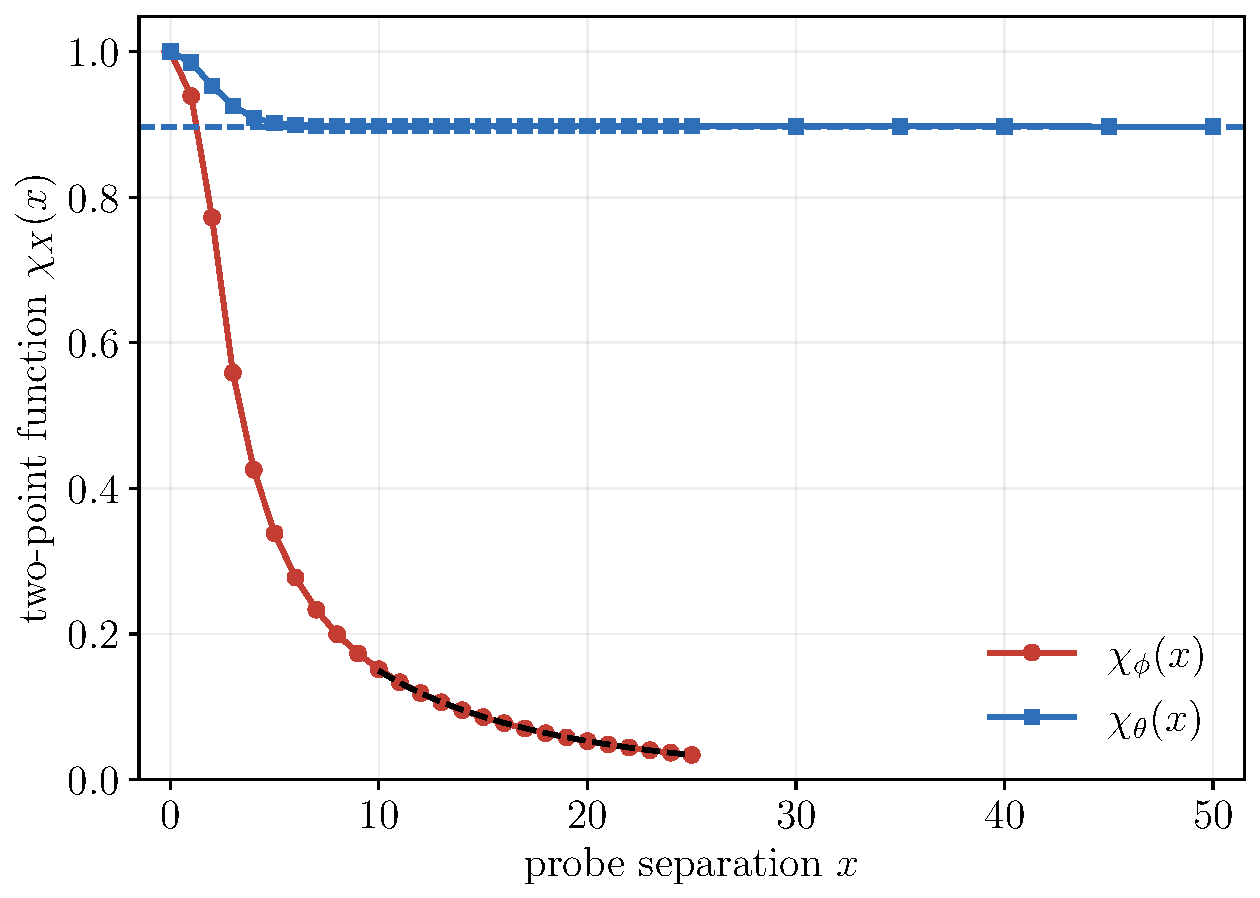
\includegraphics[width=\linewidth]{figures/paper_figS3_largeN.png}\par
\vspace{0.05cm}
{\scriptsize saddle solved numerically, $\beta=1$, $N\to1$\par}
\end{column}
\end{columns}
\onslide<3->{\tk{Gaussian: $e^{-x}$.\ \ Interactions soften it to $e^{-x^{2/3}}$}}
\end{frame}
% Notes: This part is the co-authors' controlled calculation; I only sketch it. Make theta and phi N-component vectors; the quartic interaction ~1/N; Hubbard-Stratonovich field; at large N a saddle point controls everything.
% Notes: Two-point functions of vertex operators = inserting a pair of charges (a "source") and asking how much action it costs.
% Notes: For theta: the cost saturates with distance -> constant correlator -> LRO, now in a controlled calculation (blue curve).
% Notes: Step 2: for the conjugate phi vertex, the source back-reacts: it changes the local stiffness r of the critical theory, r ~ (d_x u)^4, giving a nonlinear action with a (d_x u)^6 term.
% Notes: Step 3: balance the source against the time-derivative term and the sixth-power term: u ~ x^{2/3}, tau ~ x^{5/3}. The action grows like x^{2/3}: a stretched exponential, between a Gaussian exponential and a power law. Red curve: full numerical saddle, black dashed = x^{2/3} fit.


\begin{frame}[t]
\ft{Stretched exponential in the electron}\par
\vspace{0.4cm}
\begin{columns}[c]
\begin{column}{0.60\textwidth}
\centering
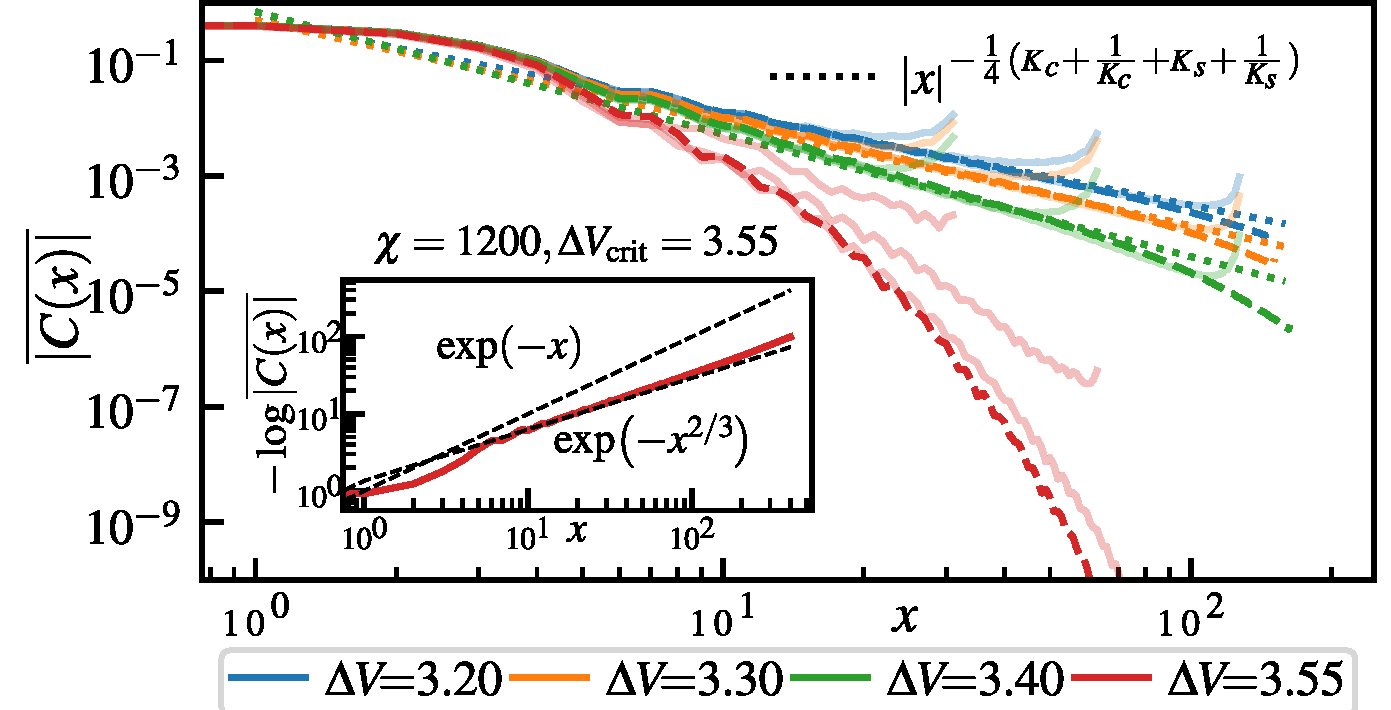
\includegraphics[width=\linewidth]{figures/paper_fig1_green.png}\par
\end{column}
\begin{column}{0.38\textwidth}
{\small $c_{\uparrow}\sim e^{i\sqrt{\pi/2}\,(\phi_c+{\color{cQCP}\phi_s}+\theta_c+\theta_s)}$\par}
\vspace{0.4cm}
\colorbox{cLL!20}{\mystrut Luttinger liquid}\\[3pt]
\hspace*{0.3cm}{\footnotesize power laws\par}
\vspace{0.35cm}
\onslide<2->{\colorbox{cQCP!15}{\mystrut Critical point}\\[3pt]
\hspace*{0.3cm}{\footnotesize ${\color{cQCP}\phi_s}$ vertex decays fastest:\par}
\hspace*{0.3cm}$C(x)\sim e^{-c\,x^{2/3}}$\par}
\vspace{0.35cm}
\onslide<3->{\colorbox{citron!40}{\mystrut Inset}\\[3pt]
\hspace*{0.3cm}{\footnotesize slope close to 2/3, moves\\ \hspace*{0.3cm}towards it with bond dimension\par}}
\end{column}
\end{columns}
\onslide<2->{\tk{Large-$N$ prediction seen at $N=1$}}
\end{frame}
% Notes: The electron itself contains the conjugate spin vertex e^{i phi_s}. So the large-N prediction should show up in the single-electron Green's function C(x) (averaged over 4 sites to remove the k_F Friedel oscillations).
% Notes: In the LL phase (blue, orange, green) all channels are power laws, envelope |x|^{-1/4(K_c+1/K_c+K_s+1/K_s)}.
% Notes: Step 2: at the QCP (red) the decay turns over to faster than any power law: the phi_s vertex dominates.
% Notes: Step 3: inset: -log C vs x on log-log: slope close to 2/3, clearly below the pure exponential. The fitted slope moves toward 2/3 with increasing bond dimension (finite-entanglement scaling, supplement). Qualitative large-N prediction holds already at N = 1.
